\section{Herramientas Criptográficas del Criptolab}

En esta sección, se analizan tres herramientas de libre distribución del repositorio Criptolab (\url{http://ingenieria.ucaldas.edu.co/gisaza/2024/ISC2024/Crypto/Cryptools.txt}), evaluando su funcionamiento, interfaz y aplicaciones prácticas.

\subsection{Herramienta de Cryptool}

Se probó la herramienta que está en línea en el repositorio \url{https://www.cryptool.org/en/cto/}. 
En este apartado se está realizando pruebas de análisis de generación de RSA con OpenSSL.

\begin{figure}[H]  % H = Here - fuerza la imagen exactamente donde aparece en el código
	\centering
	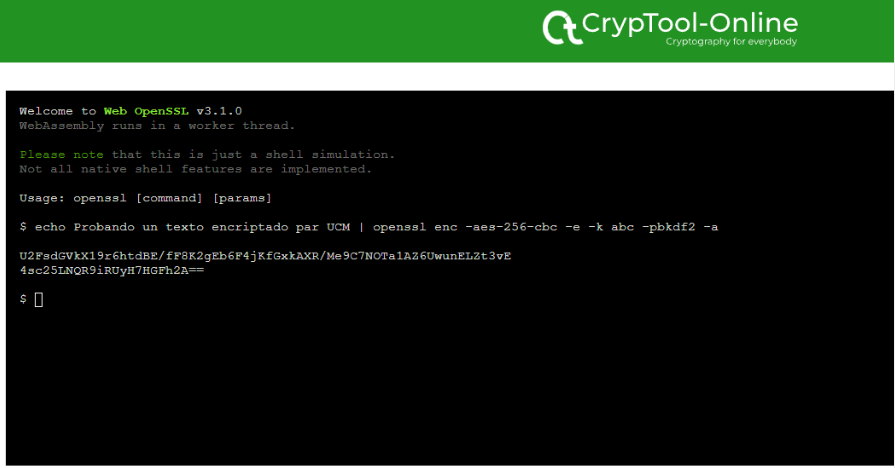
\includegraphics[width=0.75\textwidth]{./assets/img1.png}
	\caption{Interfaz principal de Cryptool}
	\label{fig:cryptool-interface}
\end{figure}

\FloatBarrier  % Evita que las figuras siguientes floten más allá de este punto

\subsection{Herramienta de Criptografía en línea}

\url{https://www.onlinecryptographytools.com/}

\begin{figure}[H]
	\centering
	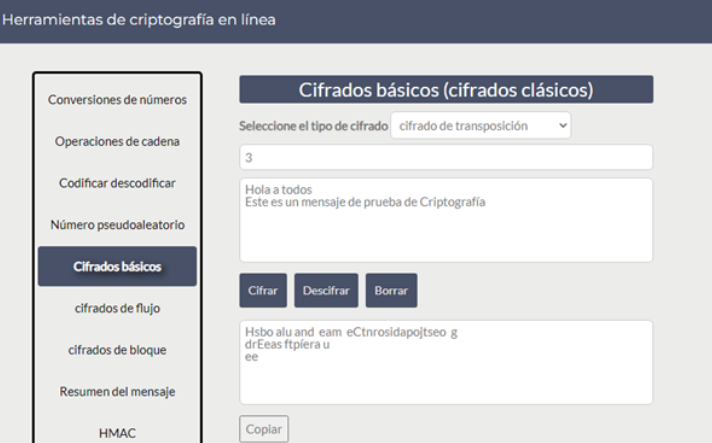
\includegraphics[width=0.75\textwidth]{./assets/img2.png}
	\caption{Herramientas de criptografía en línea}
	\label{fig:online-crypto-tools}
\end{figure}

El cifrado de transposición reordena las unidades de texto plano (como letras o grupos de letras) dependiendo del número de posición que se ingrese en el campo de texto del número de posiciones, seguido del texto a encriptar.

\begin{figure}[H]
	\centering
	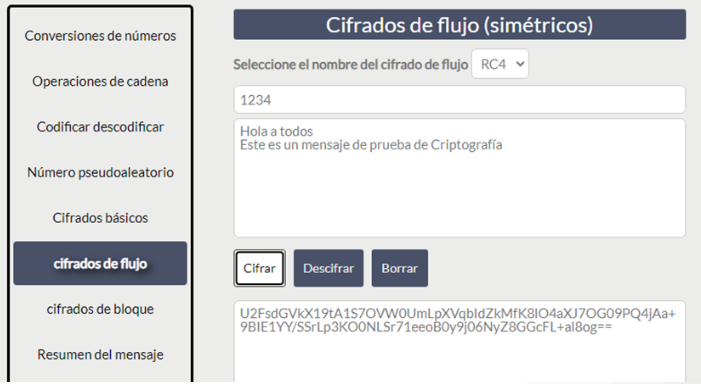
\includegraphics[width=0.75\textwidth]{./assets/img3.png}
	\caption{Demostración de cifrado por transposición}
	\label{fig:transposition-cipher}
\end{figure}

\FloatBarrier

En la sección de cifrados de flujo se ingresa una contraseña y después el texto a cifrar. A continuación se muestra el texto encriptado con contraseña:

\begin{lstlisting}[caption={Salida Hash}, label=lst:flow-cipher]
U2FsdGVkX19tA1S7OVW0UmLpXVqbIdZkMfK8lO4aXJ7OG09PQjAa+9BIE1YY/SSrLp3KO0NLSr71eeoB0y9j06NyZ8GGcFL+al8og==
\end{lstlisting}

Al realizar la desencriptación sin contraseña, esta no se ejecuta correctamente, pero al ingresar la contraseña correcta nos muestra la información original.

\begin{figure}[H]
	\centering
	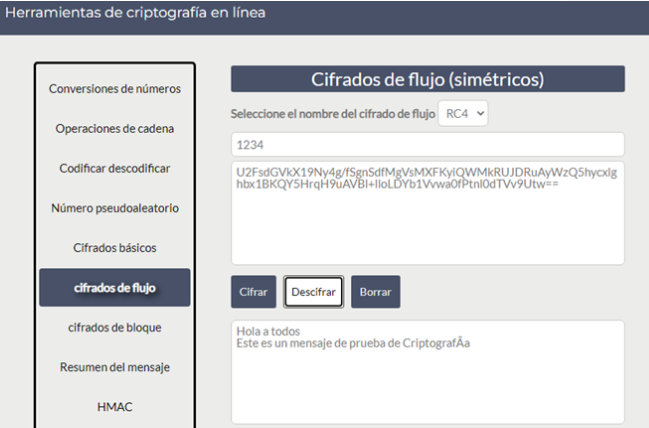
\includegraphics[width=0.75\textwidth]{./assets/img4.png}
	\caption{Proceso de desencriptación con contraseña}
	\label{fig:decryption-process}
\end{figure}

\subsubsection{Cifrados de bloque DES}

Al seleccionar el tipo de cifrado DES y colocar o generar una clave aleatoria, seguido del texto a encriptar, se genera un código encriptado con su respectiva clave. Para poder desencriptarlo debemos utilizar la contraseña ingresada anteriormente.
	
\begin{figure}[H]
	\centering
	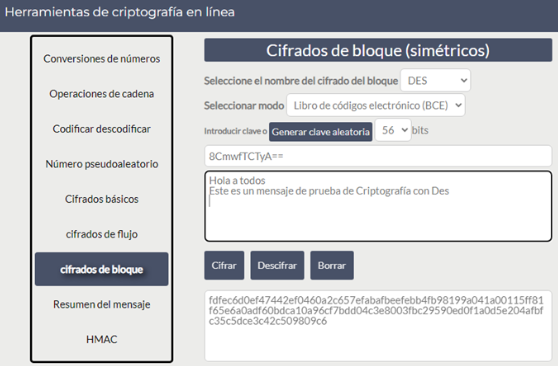
\includegraphics[width=0.75\textwidth]{./assets/img5.png}
	\caption{Interfaz de cifrado DES}
	\label{fig:des-encryption}
\end{figure}

\FloatBarrier

\subsection{Sistema de cifrado exponencial}

\href{https://www.criptored.es/software/sw_m001l.htm}{ExpoCrip: Software para Generación de Claves, Cifra y Firma RSA, ElGamal y DSS}

\begin{figure}[H]
	\centering
	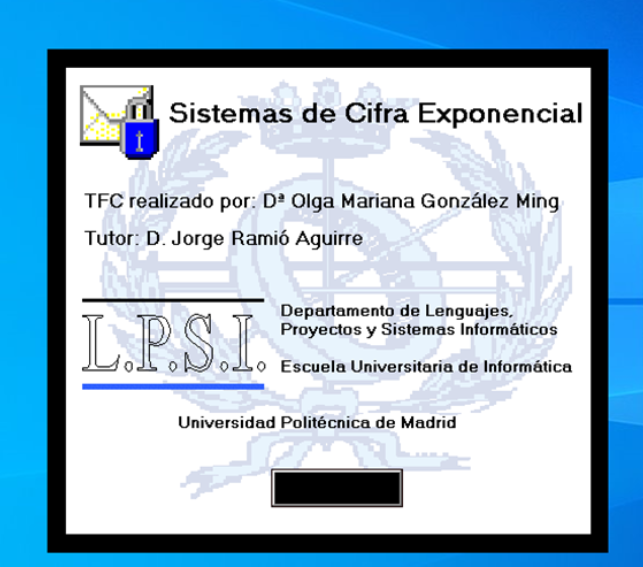
\includegraphics[width=0.75\textwidth]{./assets/img6.png}
	\caption{Interfaz del sistema de cifrado exponencial}
	\label{fig:expocrip-interface}
\end{figure}

Este sistema permite descifrar algunos parámetros de una encriptación RSA.
Inicialmente ingresamos el valor de N para conocer sus factores, los cuales representan los valores de P y Q.

\begin{figure}[H]
	\centering
	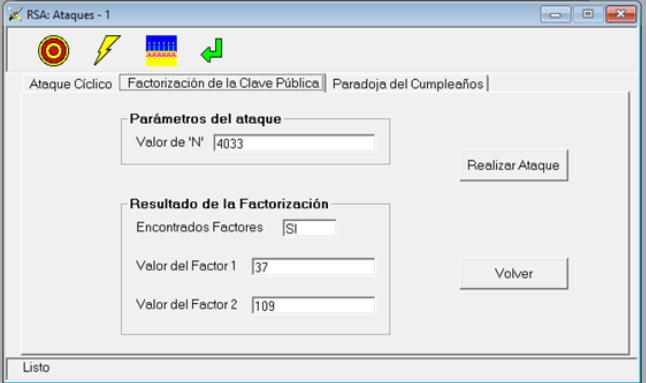
\includegraphics[width=0.75\textwidth]{./assets/img7.png}
	\caption{Factorización del valor N}
	\label{fig:n-factorization}
\end{figure}

\FloatBarrier

Ingresamos los valores de P y Q en la ventana de RSA-1 y los campos se completan automáticamente, como muestra la imagen.

\begin{figure}[H]
	\centering
	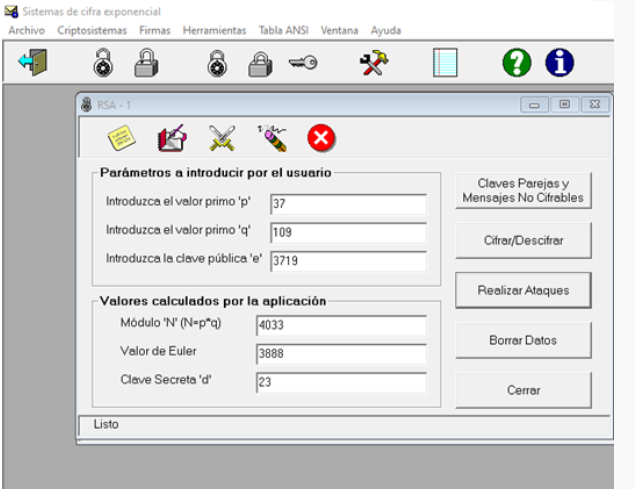
\includegraphics[width=0.75\textwidth]{./assets/img8.png}
	\caption{Introducción de valores P y Q}
	\label{fig:pq-values}
\end{figure}

Al hacer clic sobre el botón de Cifrar/Descifrar se muestra una nueva ventana:

\begin{figure}[H]
	\centering
	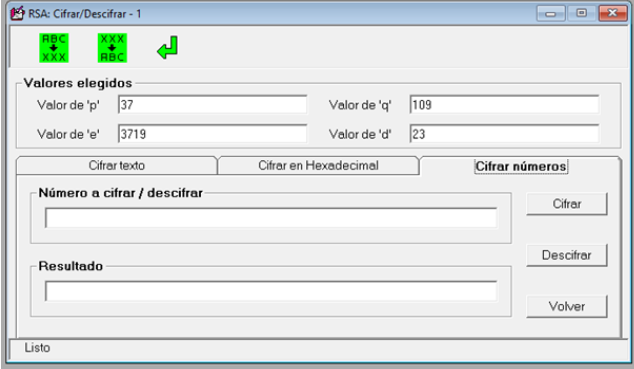
\includegraphics[width=0.75\textwidth]{./assets/img9.png}
	\caption{Ventana de cifrado/descifrado}
	\label{fig:cipher-decipher}
\end{figure}

\FloatBarrier

Seleccionamos "Cifrar Números" y en el campo de "Número o cifrar/descifrar" ingresamos:

\begin{lstlisting}[caption={Ejercicio de Cálculo}, label=lst:exercise]
Ejercicio: 8 KPR (d,N): (23,4033)
	517
	1834
	1030
	1161
	1238
	2809
	517
	3720
	2837
\end{lstlisting}
	
\begin{figure}[H]
	\centering
	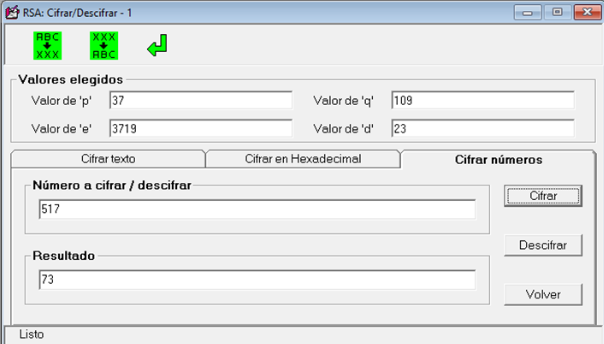
\includegraphics[width=0.75\textwidth]{./assets/img10.png}
	\caption{Entrada de valores para cifrado}
	\label{fig:cipher-input}
\end{figure}

\begin{figure}[H]
	\centering
	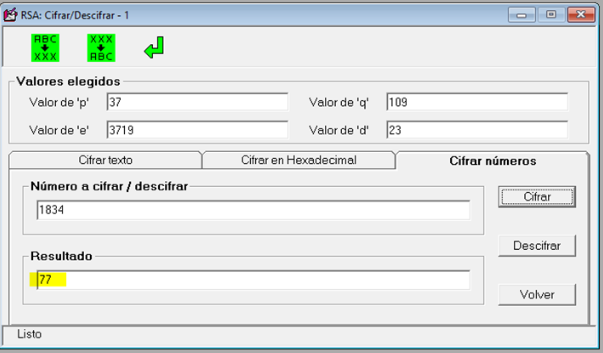
\includegraphics[width=0.75\textwidth]{./assets/img11.png}
	\caption{Proceso de cifrado exponencial}
	\label{fig:expo-cipher-process}
\end{figure}

\begin{figure}[H]
	\centering
	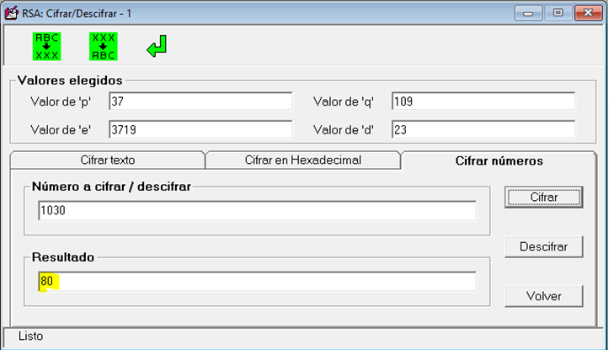
\includegraphics[width=0.75\textwidth]{./assets/img12.png}
	\caption{Resultado del cifrado exponencial}
	\label{fig:expo-cipher-result}
\end{figure}

\FloatBarrier

Como se puede observar, los resultados ya se pueden reemplazar por los valores del código ASCII, el cual nos muestra el texto desencriptado:

\begin{table}[H]
\centering
\caption{Tabla de resultado ASCII}
\label{tab:ascii-result}
\begin{tabular}{|c|c|c|}
\hline
\textbf{C} & \textbf{N} & \textbf{Texto} \\
\hline
517  & 73 & I \\
1834 & 77 & M \\
1030 & 80 & P \\
1161 & 82 & R \\
1238 & 69 & E \\
2809 & 83 & S \\
517  & 73 & I \\
\hline
\end{tabular}
\end{table}

